\documentclass[a4paper,12pt]{article}
\usepackage{fullpage, float, graphicx}
\title{CS26410 Report 3\\
Hide and Seek}
\author{Chris Savill\\\texttt{chs17@aber.ac.uk}}
\begin{document}
\maketitle
\newpage
\tableofcontents
\newpage

\section{Description of algorithms used}

\subsection{Depth-First-Search (DFS) algorithm}
\noindent The DFS algorithm is used to aid in exploring a whole area. The algorithm requires that a stack is used to store the path along which the robot has travelled to get to its current cell on the occupancy grid. The reason it acts as a DFS is because the algorithm keeps the robot searching further rather than restricting it to searching a close area to a start point and then working out.

\begin{figure}[H]
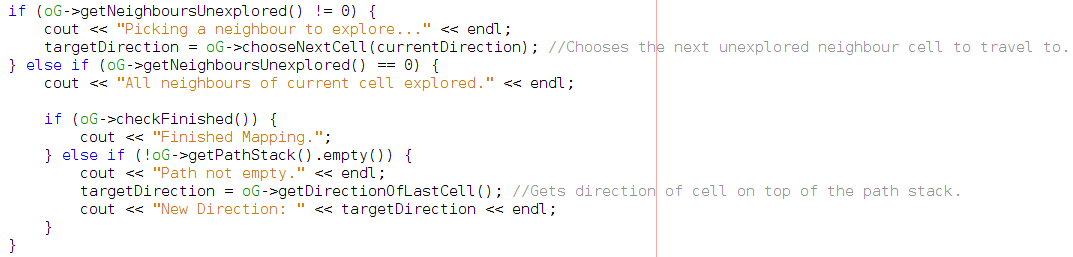
\includegraphics[scale=0.8]{DFS_SS.png}
\caption{Snapshot of DFS code.}
\end{figure}

\vspace{5mm}
\noindent The algorithm has a way of determining if the mapping of an area is complete. The check is a function that evaluates if every cell that has been explored and has no obstacle present, has no unexplored neighbours. If this return true then the search and mapping is complete so the path stack is emptied thus finishing the mapping task.

\begin{figure}[H]
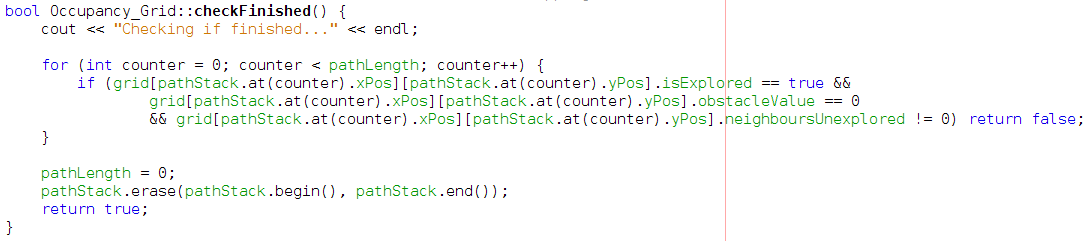
\includegraphics[scale=0.55]{Check_Finished_SS.png}
\caption{Snapshot of check finished function code.}
\end{figure}

\vspace{5mm}
\noindent The way in which the algorithm chooses which direction to continue in at each cell is quite simple. If the cell directly in front of the robot is explorable, the robot will continue in that direction. This was implemented as it speeds up the search because the robot takes a long time to turn. If the cell in front has an obstacle present, a random number is generated that correlates to each of the 4 directions it can travel and checks if that cell is unexplored and has no obstacle present. This random number generator is constantly generated until a cell that is unexplored and is explorable is chosen.

\subsection{Localisation algorithm}
\noindent The localisation algorithm is use to determine whether the robot is within the occupancy grid and if so, where. The algorithm itself works as follows. A new temporary occupancy grid is created for the robot to use for its mapping of its immediate area. Once the immediate area is scanned the temporary grid is compared to all areas of the original occupancy grid. The comparison algorithm uses a 2 for loops to ensure that the temporary grid area is compared to all possible areas of the original grid. The temporary grid is compared to areas of the same size and each individual cell is compared with the corresponding cell of the area being compared with in the original grid.

\begin{figure}[H]
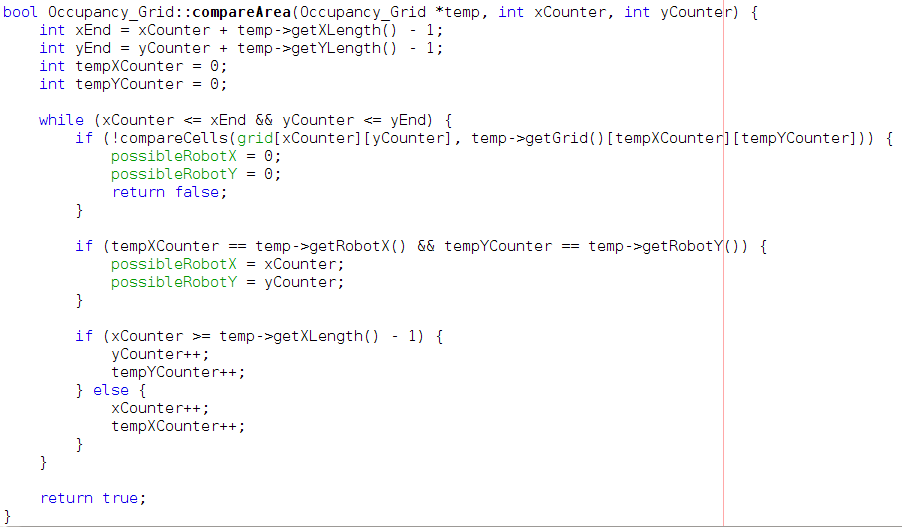
\includegraphics[scale=0.65]{Compare_Area_SS.png}
\caption{Snapshot of compare area function code.}
\end{figure}

\vspace{5mm}
\noindent If the localisation of that area is unsuccessful then the algorithm exits telling the user that the robot is not within the original occupancy grid area. If there is more than 1 place the robot could possible be, the robot uses the DFS algorithm and moves to the next unexplored cell and tries to localise with the additional information gathered. If the comparison algorithm determines that there is only one possible place for the robot to be, the robot switches to using the original occupancy grid and is localised to the area it was found in. As localisation requires that an original occupancy grid exists to compare with, there is a boolean value that tell the robot that it mapped successfully so localisation can be attempted.

\begin{figure}[H]
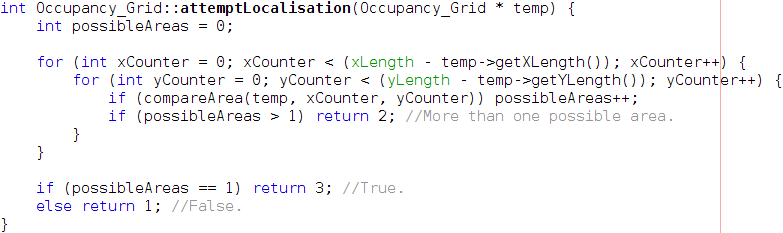
\includegraphics[scale=0.75]{Attempt_Localisation_SS.png}
\caption{Snapshot of attempt localisation function code.}
\end{figure}

\subsection{Hiding algorithm}
\noindent The hiding algorithm consists of 3 parts; the first part involves finding the best place to hide, the second part involves finding the shortest path to that position and the third part involves getting the robot to travel along that path to its hiding location. The hiding function can only be accessed if the localisation of the robot is successful. In order to find the best hiding spot for the robot the algorithm first searches for empty, explored cells and checks if the have 3 walls around them, if none can be found does the same but looks for 2 walls and then 1. 

\begin{figure}[H]
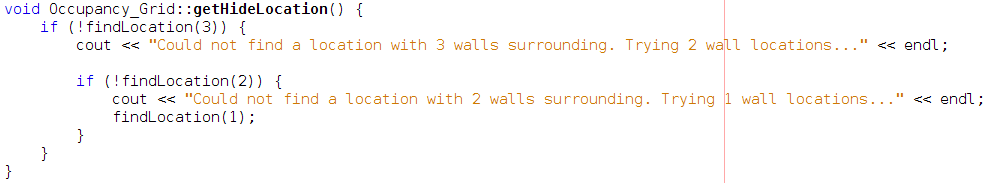
\includegraphics[scale=0.6]{Get_Hide_Location_SS.png}
\caption{Snapshot of code that calls function to search for a hiding place.}
\end{figure}

\begin{figure}[H]
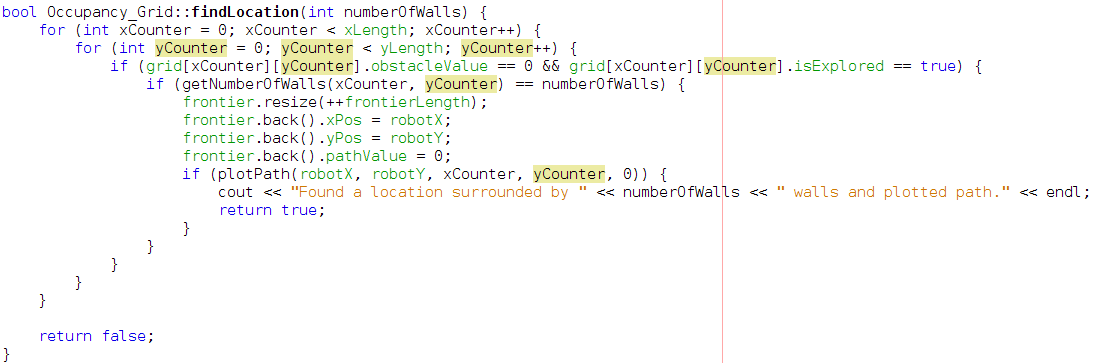
\includegraphics[scale=0.55]{Find_Location_SS.png}
\caption{Snapshot of function that tries to find a hiding location and plot a path using other functions.}
\end{figure}

\vspace{5mm}
\noindent The path finding algorithm is a simple A* search that keeps track of the distance/cost so far and the distance/cost left. The search tries to find the shortest path possible as the search is guided in the direction of the target cell and the total goal value is underestimated not overestimated so it is admissible. Once the path as been plotted from the robot's current location to its hiding location, the robot moves cell by cell along its path until the path stack is empty, at which point the robot should be at its hiding location.

\begin{figure}[H]
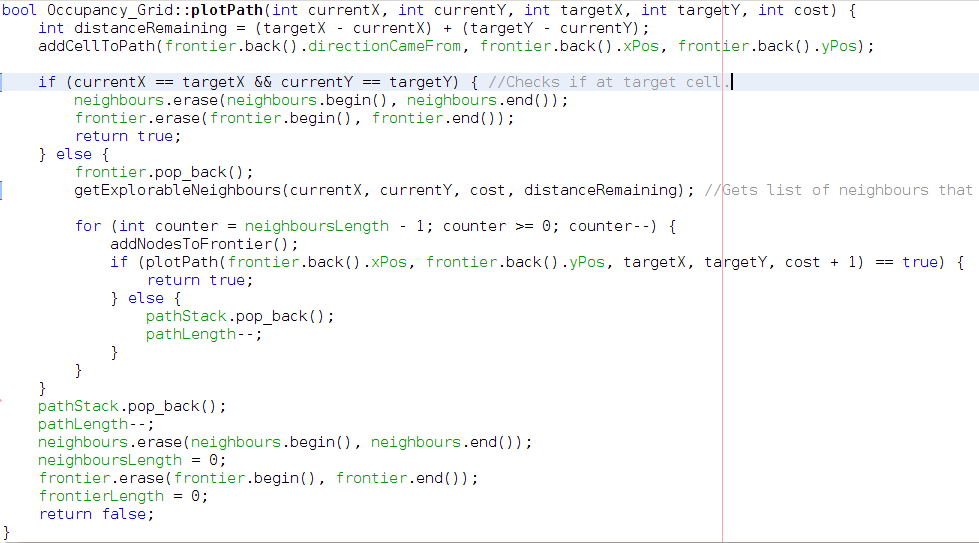
\includegraphics[scale=0.6]{Plot_Path_SS.png}
\caption{Snapshot of function that uses performs an A* search with the aid of other functions.}
\end{figure}

\subsection{Seeking algorithm}
\noindent The seeking algorithm is very simple, if the robot localised successfully, the robot will perform a DFS of the whole pre-explored area, if however any cells that did not contain an obstacle on the original occupancy grid are detected to have an obstacle, then the DFS finishes and the anomaly is stated to the user, thus finishing the seeking function.

\begin{figure}[H]
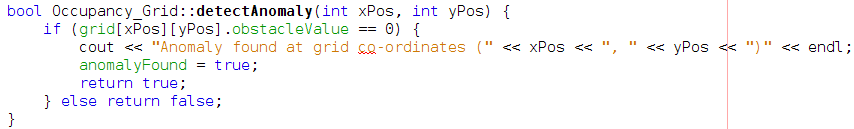
\includegraphics[scale=0.65]{Detect_Anomaly_SS.png}
\caption{Snapshot of function that determines if an anomaly has been found.}
\end{figure}

\section{Trial runs}

\subsection{Simulated trial runs}
\noindent In order to perform real world trials, the robot program first had to be tested through the use of Player/Stage. Before testing proceeding onto real world trials, the robot had to successfully map the whole area of the simulated world provided. Many of the runs were unsuccessful resulting in the robot crashing at some point. Below is a series of screen shots of one of the successful trials for mapping:

\vspace{5mm}
\noindent Key:
\begin{table}[H]
\begin{tabular}{| l | l |}
	\hline
	\textbf{Icon} & \textbf{What it represents}
	\\\hline
	\# & Obstacle present
	\\\hline
	\textasciitilde & Unexplored cell
	\\\hline
	R & Robot's current location
	\\\hline
	 & An empty cell represents an explored cell with no obstacle present.
	\\\hline
\end{tabular}
\end{table}

\begin{figure}[H]
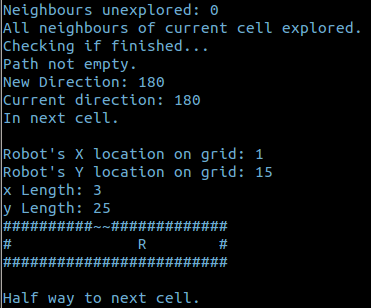
\includegraphics[scale=1.0]{RunT1.png}
\caption{Screen shot of the terminal window corresponding to the screen shot below. Having mapped the the bottom area and hitting a dead end, the robot return along its path to the next available unexplored cell.}
\end{figure}

\begin{figure}[H]
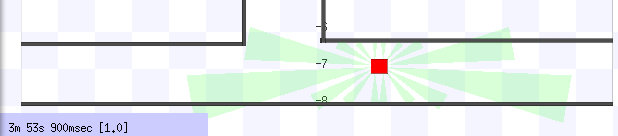
\includegraphics[scale=0.9]{RunS1.png}
\caption{Screen shot of the Stage window corresponding to the screen shot above.}
\end{figure}

\begin{figure}[H]
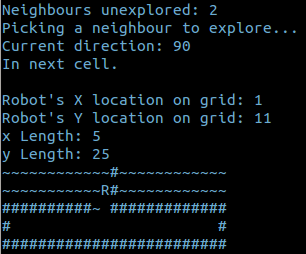
\includegraphics[scale=1.0]{RunT2.png}
\caption{Screen shot of the terminal window corresponding to the screen shot below. Having found the next unexplored cell the robot starts to travel and map upwards.}
\end{figure}

\begin{figure}[H]
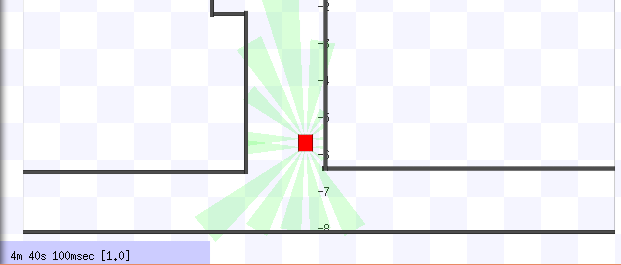
\includegraphics[scale=0.9]{RunS2.png}
\caption{Screen shot of the Stage window corresponding to the screen shot above.}
\end{figure}

\begin{figure}[H]
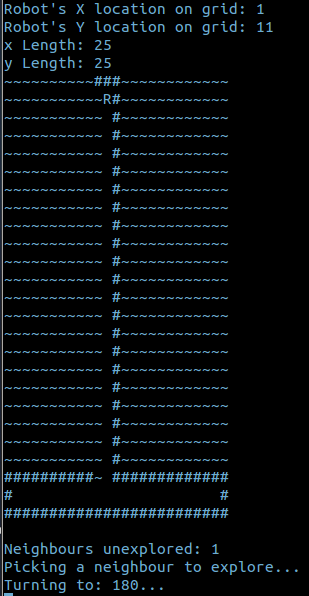
\includegraphics[scale=1.0]{RunT3.png}
\caption{Screen shot of the terminal window corresponding to the screen shot below. Having reached the top the robot turns left as it is the only neighbour cell unexplored.}
\end{figure}

\begin{figure}[H]
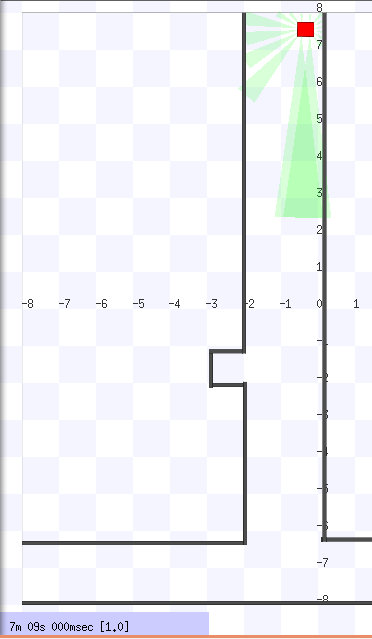
\includegraphics[scale=0.9]{RunS3.png}
\caption{Screen shot of the Stage window corresponding to the screen shot above.}
\end{figure}

\begin{figure}[H]
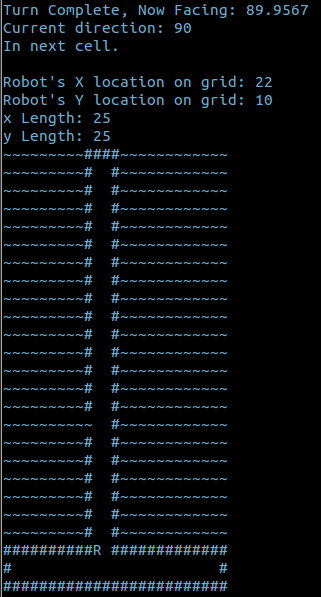
\includegraphics[scale=1.0]{RunT4.png}
\caption{Screen shot of the terminal window corresponding to the screen shot below. Having scanned the left side all the way back to the pre-explored area, the robot turns to travel back along its path to the next unexplored cell.}
\end{figure}

\begin{figure}[H]
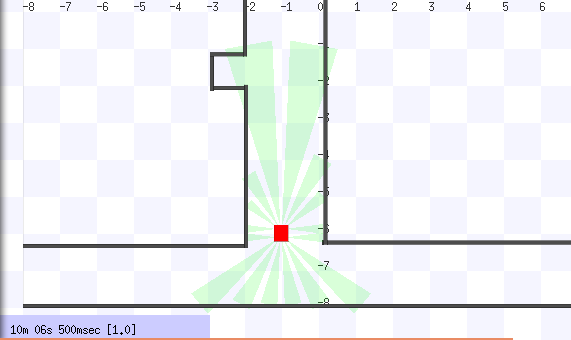
\includegraphics[scale=0.9]{RunS4.png}
\caption{Screen shot of the Stage window corresponding to the screen shot above.}
\end{figure}

\begin{figure}[H]
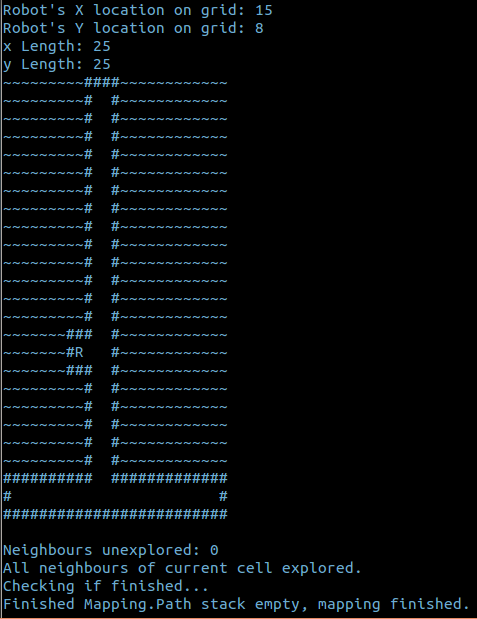
\includegraphics[scale=1.0]{RunT5.png}
\caption{Screen shot of the terminal window corresponding to the screen shot below. Having reached a dead end, the robot evaluates if it has any cells left to explore. As it evaluates there are none, the mapping is declared finished.}
\end{figure}

\begin{figure}[H]
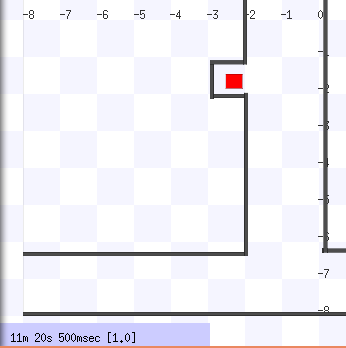
\includegraphics[scale=0.9]{RunS5.png}
\caption{Screen shot of the Stage window corresponding to the screen shot above.}
\end{figure}
\subsection{Real world trial runs}

\section{Discussion of trial run results}
\noindent At the start it was expected that a lot of the simulated trial runs would finish prematurely due to a robot crash. This was in fact the case. Most of the time the robot would crash when turning and usually it was at the bottom of the simulated world where the robot tries to explore the upper section. Once it occurred that a 60cm by 60cm cell space was not sufficient to give the robot space to turn (explained in the evaluation section below) and this was amended to 70cm by 70cm cells, the robot managed to avoid getting too close to the walls so did not have problems when turning and was then able to complete a full successful map of the simulated area. This same result was replicated again when the function implemented to check that the robot had finished mapping needed testing.

\vspace{5mm}
\noindent In terms of real world results, 

\section{Evaluation of work done}

\subsection{Positive parts}
\noindent The mapping algorithm implemented ensures that all explorable cells are explored due to the nature of a depth-first-search. The accuracy of the mapping is also very good as shown in the simulated trial run. As the mapping is very accurate due to only scanning a maximum of 8 cells around the robot at any given time (to reduce errors with sonar spread at longer ranges), there is no need to apply a threshold to the values. This helps improves efficiency as there is one less task to run.

\vspace{5mm}
\noindent The robot program implemented the way it is would work very well in a square world where all shapes are square-like. This is because the robot turns to the angles 0, 90, 180 and 270 degrees and no others. The path plotting algorithm is quite simple and as it uses an A* search, the path required to get the robot to its hiding location should be found quite fast without too many extra nodes being expanded. Also because the robot can keep track of a path along which it has travelled and return along, the path found by the A* algorithm is simply loaded into the robot for it to follow to get to its destination.

\vspace{5mm}
\noindent The robots localisation algorithm is also simple but enables the robot to localise as soon as possible and also notify the user that localisation is unsuccessful as soon as possible. This is great as a robot that has limited battery power wants to avoid draining power where possible moving around.

\subsection{Negative parts}
\noindent The main negative part about the robot program implemented is that the robot is very deliberative and is constrained to working in a square environment. As the robot only turns to the 0, 90, 180, 270, the robot is very limited in moving around environments. The robot is also constrained in moving forwards not backwards and at set distances, this again limits the robots capabilities with adapting to different environments. All of these problems exist mainly because of the deliberative nature of of the program implemented.

\vspace{5mm}
\noindent Due to the robot not having any real reactive features implemented, it totally relies on everything working properly. For instance, if the robot does not turn to the correct angle, the robot may move into an obstacle. Also due to the robot using odometry to determine it location, relying on the revolution of the wheels for the co-ordinate and yaw changes, there is possible way code can be used to correct any mistakes we as human can see when the robot truly believes it has it its targets. The robot also doesn't have any way of dealing with inclinations.

\subsection{Hardest parts}
\noindent The hardest part to implement was the mapping algorithm as it is a complex task to accomplish. Deciding how many and which sensors to use was a problem as well as figuring/estimating the angles and error bounds for each sensor. Also, regarding the sensors, the range at which the values returned would be considered accurate was an aspect of the project that took some thought. It was decided to just use ranges that would enable one cell in each direction to be scanned reliably including the diagonal/corner cells (8 cells around the robot in total). Detecting corners was a big problem that needed a lot of trial and error to get reasonably working.

\vspace{5mm}
\noindent With regards to problems encountered with using a real robot, the main problem was the robots believing they had turned to the specified angle wanted when in reality they had not. This needed a lot of trial of error with changing the PGAIN value using when calculating the turn rate for the robot. Even at that point each turn would not produce the same result so the robot would easily be able to produce different results with each run, sometimes resulting in a crash.

\subsection{What would be done differently}
\noindent An attempt to implement a reactive robot would be made to enable the robot to adaptive to a changing environment more effectively and avoid crashing better. If a reactive system was implemented, it may be a lot more complex (reason for not using this approach) but would allow the robot to have more freedom and deal with obstacles appearing right next to it (such as an object moving into its path etc). It would also be easier for the robot to avoid being too close to walls (or at least correct to get a minimum distance from the walls) and thus avoid crashing when it turns. However, giving the robot more freedom with movement would make it more difficult to map as it would be harder to determine where the robot would be located on the grid so this may still not be a real viable option.

\vspace{5mm}
\noindent Another place where things would be done differently would be in the testing area. Testing the robot in different simulated environments would help to produce a robot that could function better in various kinds of environments (be more versatile). Also the same goes for real world testing/trials.
\end{document}